\section{Designdokumentation}
\subsection{Designklassediagram}
\begin{figure}[H]
            \centering
            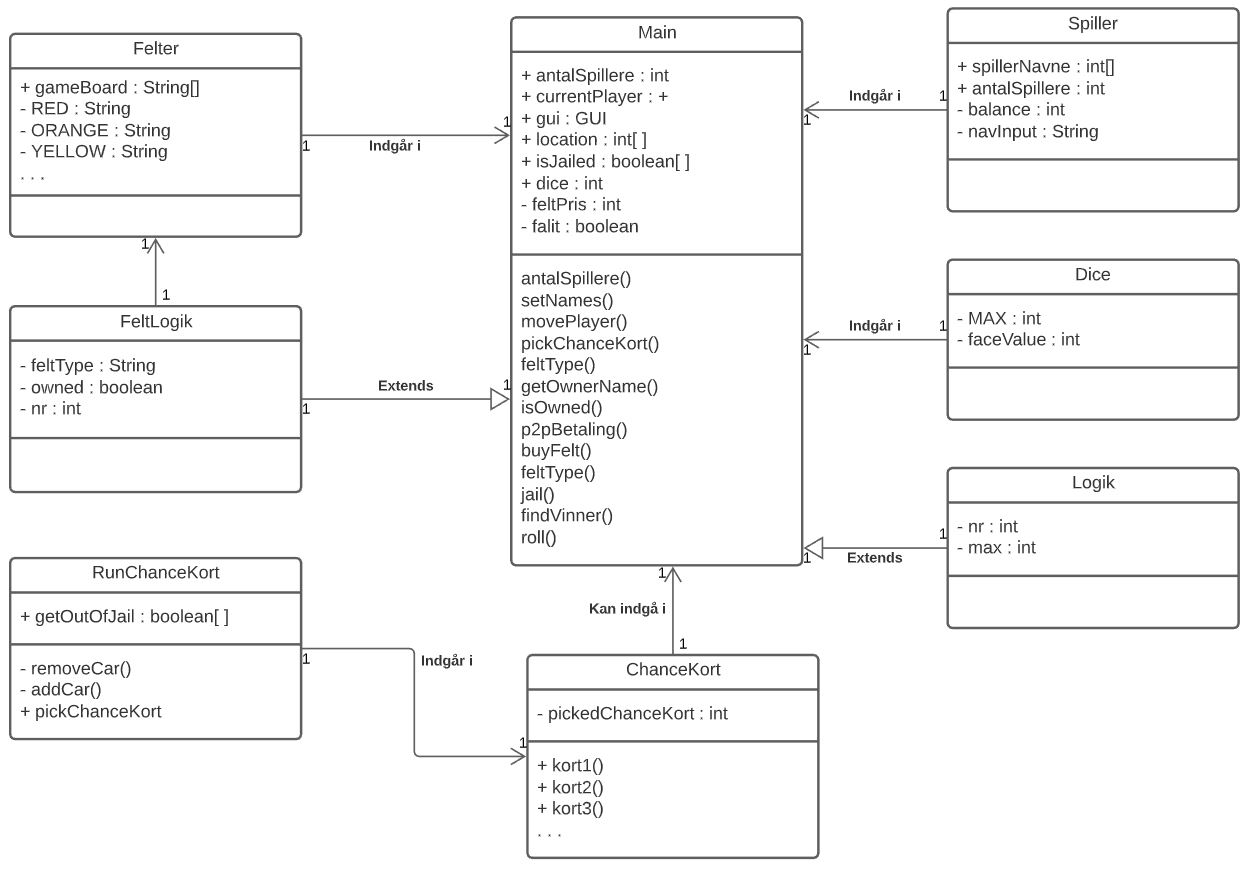
\includegraphics[width=14cm]{figures/designKlasseDiagram.JPG}
            \caption{Designklassediagram}
        \end{figure}
        
Design-klassediagrammet benyttes i alt sin simpelhed til at give et  hurtigt og overordnet overblik over systemets klasser og hvordan de er relateret til hinanden.  Klassediagrammet viser hvilke metoder og attributter der tilhøre den enkelte klasse, samt hvilke klasser der er associeret med hinanden. 
Ud fra klassediagrammet kan det ses, at der er en "Main" klasse, den klasse består af en længere række attributter som f.eks. antalSpillere, Gui, dice osv. Desuden er klassen tildelt samtlige metoder deriblandt, setName, movePlayer, feltType m.m. Main klassen er associeret med præcis 5 klasser, hvor netop Main indgår. Endvidere kan det ses at klasserne FeltLogik og Logik er nedarvet af Main, hvad også kaldes subclass og superclass. Det vil sige en klasse som kan gøre brug af variable fra den klasse, som den er nedarvet fra. 

Vi gør ikke brug af abstract klasser. En abstract klasse er en klasse, hvor metoderne er "låste" til klassen. Det kan bruges i situationer, hvor man ikke ønsker at metoderne skal kunne tilgås udefra klassen selv. 

Vi kunne også have gjort brug af polymorfi, da vi lavede felterne. Vi valgte dog at have alle felterne i en klasse, da vi vurderede, at det ikke ville fylde sønderligt meget. Ved brug af polymorfi kan man tilgå 2 metoder, som hedder det samme, fra 2 forskellige klasser og skelne imellem dem. 
        
\subsection{Sekvensdiagram}
    \begin{figure}[H]
        \centering
        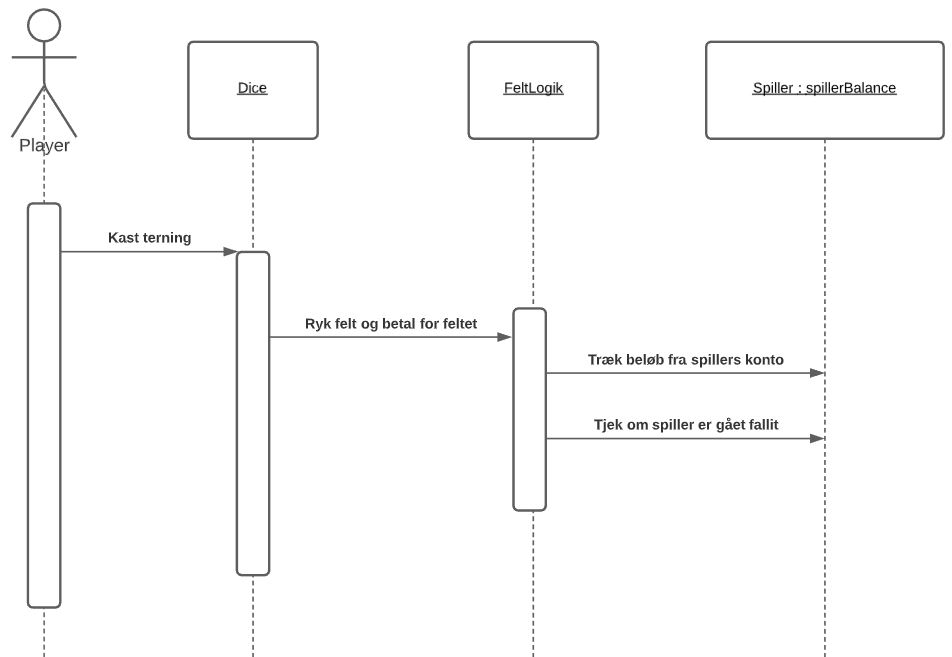
\includegraphics[width=15cm]{figures/systemSekvensDiagram.JPG}
        \caption{Sekvensdiagram}
        \emph{Sekvensdiagrammet illustrerer hvordan spillet virker som helhed}
    \end{figure}
    
Sekvensdiagrammet viser metodekaldene mellem forskellige objekter henover en arrangeret tidslinje. I diagrammet er der i øvrigt opmærksomhed på rækkefølgen, hvormed meddelelserne sendes til objekterne. 
Objekterne er illustreret ved lodrette streger som f.eks. "Kast terning" og "Træk beløb fra spillers konto", desuden viser den lodrette orientation også tiden. Hvert objekt sender meddelelserne fra et objekt til et andet, hvor der er givet en operation og et paramenternavn.  

\subsection{Brugergrænseflade}

Brugergrænsefladen er måden hvorpå brugeren benytter sig af systemet. Det er netop bindleddet mellem systemet og dets brugere. Der er særligt 2 punkter som brugergrænsefladen tilbyder; Inddata og uddata. Inddata tillader brugeren at styre systemet og uddata kan informere brugeren, også kaldt feedback. Disse former for data kan f.eks.vise brugernes kommandoer og systemets svar på de givne kommandoer. Dog er brugergrænsefladen helt principielt den facade brugeren har kontakt med som tastaturet og musen.

\newpage
\subsection{GRASP-mønstre}

I henhold til GRASP-mønstrene har vi forsøgt at overholde low coupling og high cohesion. Altså at koden er veldefineret i forhold til ansvarsområde, uden at være for afhængig af hinanden. Det har vi i spillet gjort ved at klasserne styrer hver deres del. Eksempelvis er Dice-klassen den samme som fra de foregående CDIO-projekter, med den éne arbejdsopgave, at stå for et tilfældigt output fra 1-6